\documentclass[11pt,a4paper]{article}
    \usepackage[margin=2.5cm]{geometry}
    \usepackage{enumitem}
    \usepackage{hyperref}
    \usepackage{tikz}
    \usetikzlibrary{arrows.meta,positioning,shapes.geometric}
    \title{Statistical Plotting Tools}
\author{Jordi Vill\`a-Freixa \texttt{<jordi.villa@uvic.cat>}}
    \date{\today}

    \tikzset{
      methodbox/.style={
        rounded corners=6pt,
        draw=blue!50!black,
        line width=0.9pt,
        fill=blue!6,
        minimum width=13cm,
        text width=11.8cm,
        align=left,
        inner sep=8pt
      }
    }

    \begin{document}
    \maketitle

    \section*{Scope}
    This folder contains compact teaching material for probability distributions and simple exploratory histograms from CSV data.

    \section*{Material in this folder}
    \begin{itemize}[leftmargin=*]
\item \texttt{distributions.ipynb}
\item \texttt{simple\_histogram.py}
    \end{itemize}

    \section*{Method summary}
    \begin{itemize}[leftmargin=*]
\item \textbf{Probability distribution visualization}. The notebook illustrates analytical probability density functions and their parameter dependence.
\item \textbf{Histogram generation from tabular data}. The Python script reads a CSV file, coerces one selected column to numeric values, prints summary statistics, and plots a histogram.
\item \textbf{Basic descriptive statistics}. Before plotting, the histogram script computes summary metrics such as count, mean, and quantiles.
    \end{itemize}

    \section*{Method scheme}
    Figure~\ref{fig:summary} is drawn directly in LaTeX with TikZ. It is a compact conceptual map of the main workflows discussed in this folder.

    \begin{figure}[ht]
    \centering
    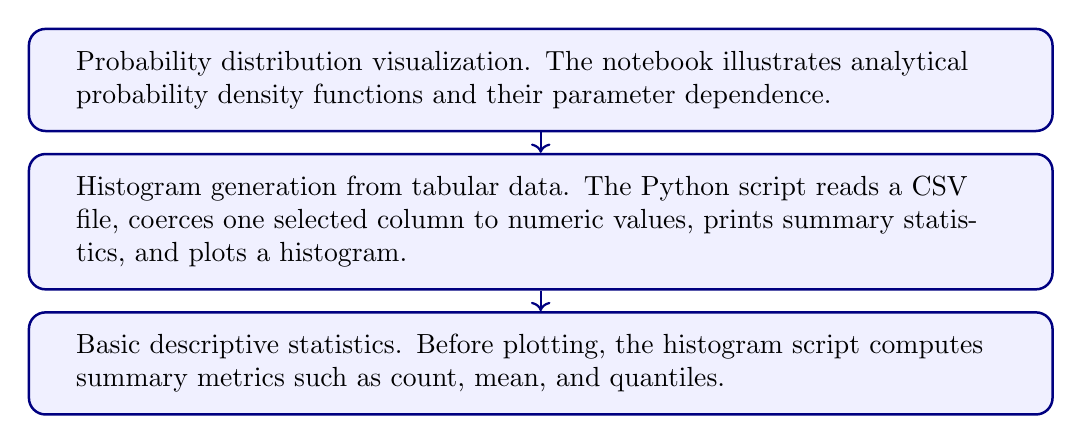
\begin{tikzpicture}[x=1cm,y=1cm]
    \node[methodbox] (m0) at (0,0.0) {Probability distribution visualization. The notebook illustrates analytical probability density functions and their parameter dependence.};
    \node[methodbox] (m1) at (0,-1.8) {Histogram generation from tabular data. The Python script reads a CSV file, coerces one selected column to numeric values, prints summary statistics, and plots a histogram.};
    \node[methodbox] (m2) at (0,-3.6) {Basic descriptive statistics. Before plotting, the histogram script computes summary metrics such as count, mean, and quantiles.};
    \draw[->, thick, color=blue!50!black] (m0.south) -- (m1.north);
    \draw[->, thick, color=blue!50!black] (m1.south) -- (m2.north);
    \end{tikzpicture}
    \caption{Conceptual scheme for the methods in the statsTools folder.}
    \label{fig:summary}
    \end{figure}

    
\bibliographystyle{plain}
\bibliography{../references}

\section*{Disclaimer}
These documents were generated with the assistance of ChatGPT 5.4. The material has been reviewed by the author before inclusion in this repository, but it is not free from possible errors.

\end{document}